\section{Results and Findings}
    \begin{frame}{Simple Answer}
        \begin{columns}
        \begin{column}{0.5\textwidth}
        \begin{itemize}
            \item<1-> A brutal but informative plot
            \item<2-> In the long run, commodity prices do grow faster than
inflation
            \item<3-> Compared to consumption goods, commodity prices are crazily fluctuating, so not much we can say about short term
        \end{itemize}
        \end{column}
        \begin{column}{0.5\textwidth}  %%<--- here
            \begin{center}
             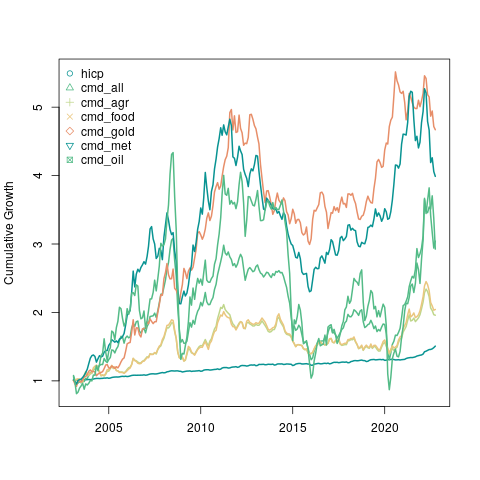
\includegraphics[width=\textwidth]{../../figures/cumgrowth.png}
             \end{center}
        \end{column}
        \end{columns}
    \end{frame}

    \begin{frame}{Exploring Inflation}
        \begin{columns}
        \begin{column}{0.5\textwidth}
        \begin{itemize}
            \item<1-> The plot shows 12-month growth rates of prices of groups of consumption goods
            \item<2-> Some groups, like durables and services, shows volatile price changes
            \item<3-> The overall pace of growth in the all-item and core prices are quite steady
        \end{itemize}
        \end{column}
        \begin{column}{0.5\textwidth}  %%<--- here
            \begin{center}
             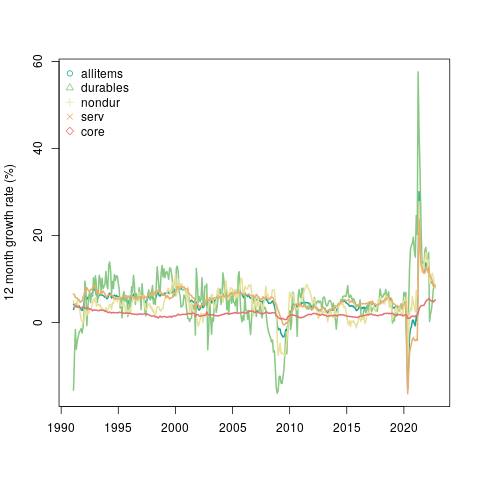
\includegraphics[width=\textwidth]{../../figures/growth12.png}
             \end{center}
        \end{column}
        \end{columns}
    \end{frame}


    \begin{frame}{Correlations?}
        \begin{columns}
        \begin{column}{0.5\textwidth}
        \begin{itemize}
            \item<1-> The first column is of the most interests, showing the correlation between HICP and commodity price growths in different groups
            \item<2-> All of the correlations here are positive, but not too strong
            \item<3-> Oil price is most correlated to inflation among all groups, which is consistent with common sense
        \end{itemize}
        \end{column}
        \begin{column}{0.5\textwidth}  %%<--- here
            \begin{center}
             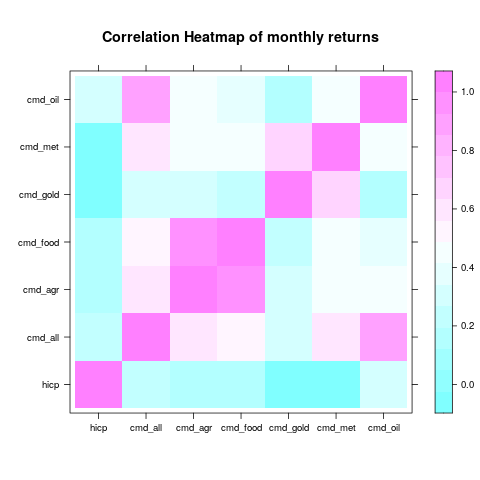
\includegraphics[width=\textwidth]{../../figures/heatmapcmd.png}
             \end{center}
        \end{column}
        \end{columns}
    \end{frame}


    % \begin{frame}{Introducing Stock Index}
    %     \begin{columns}
    %     \begin{column}{0.7\textwidth}
    %     \begin{itemize}
    %         \item<1-> The first column is of the most interest, showing the correlation between HICP and commodity price growths in different groups
    %         \item<2-> All of the correlations here are positive, but not too strong
    %         \item<3-> Oil price is most correlated to inflation among all groups, which is consistent with common sense
    %     \end{itemize}
    %     \end{column}
    %     \begin{column}{0.3\textwidth}  %%<--- here
    %     \setstretch{1}
    %         \begin{figure}[t]
    %         \subfloat{%
    %         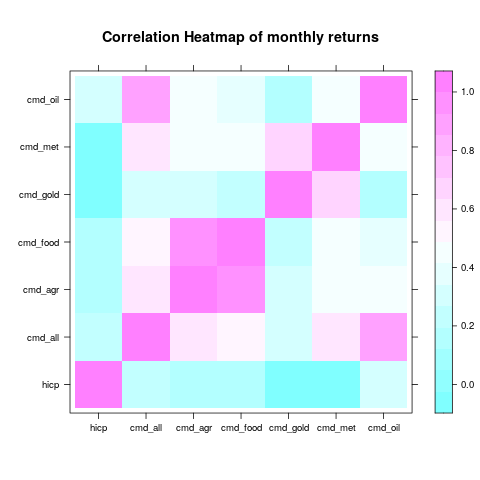
\includegraphics[clip,width=0.6\textwidth]{../../figures/heatmapcmd.png}}\\
    %         \subfloat{%
    %         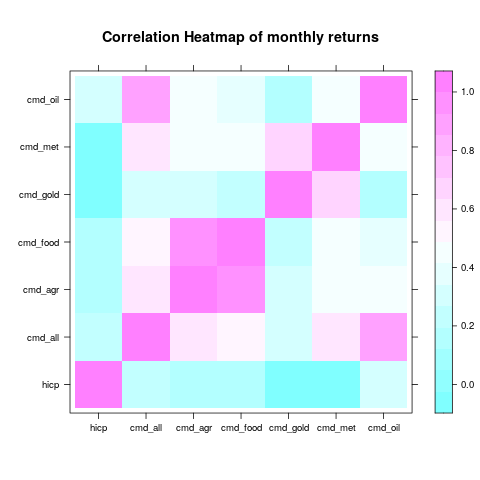
\includegraphics[clip,width=0.6\textwidth]{../../figures/heatmapcmd.png}} \\
    %         \subfloat{%
    %         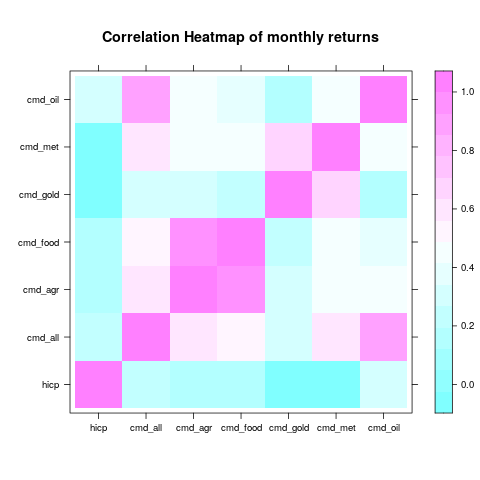
\includegraphics[clip,width=0.6\textwidth]{../../figures/heatmapcmd.png}}
    %         \end{figure}
    %     \end{column}
    %     \end{columns}
    % \end{frame}
    
    \begin{frame}{Correlations?}
        \begin{itemize}
            \item<1-> From Figure~\ref{fig:sfig2}, we can see that before 2004, there was no obvious consistency between the stock and commodity indices, while after 2004, the local peaks and bottoms often coincide
            \item<2-> In both periods of consideration, the stock index showed weakly positive correlations with the commodity index, while in the longer term this interaction was a bit stronger
            \item<3-> Durables and non-durables are most strongly correlated to S\&P 500. The longer term sees stronger correlations for durables
        \end{itemize}
        
        \begin{figure}[h!]
        \begin{subfigure}{0.27\textwidth}
          \centering
          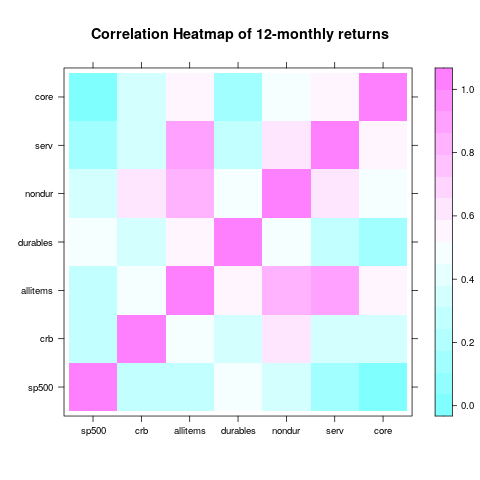
\includegraphics[width=\linewidth]{figures/heatmapsp500.png}
          \caption{Correlation, 12-months}
          \label{fig:sfig1}
        \end{subfigure}%
        \begin{subfigure}{0.27\textwidth}
          \centering
          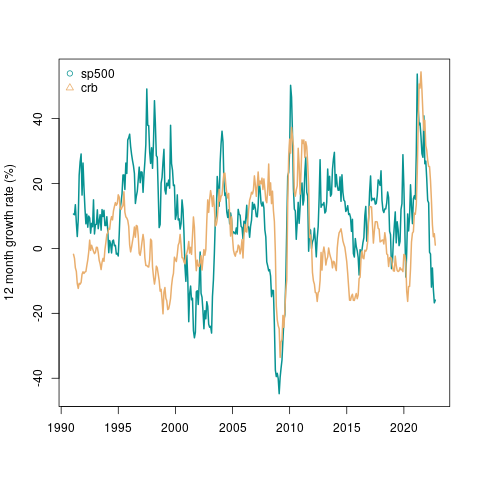
\includegraphics[width=\linewidth]{figures/cumgrowth12.png}
          \caption{S\&P 500 v.s. CRB\\ 12-months}
          \label{fig:sfig2}
        \end{subfigure}
        \begin{subfigure}{0.27\textwidth}
          \centering
          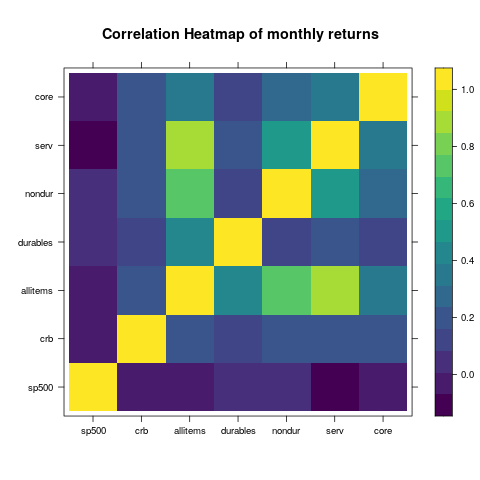
\includegraphics[width=\linewidth]{figures/heatmappce.png}
          \caption{Correlation, 1-month}
          \label{fig:sfig3}
        \end{subfigure}
        \label{fig:SP}
        \end{figure}
    \end{frame}